\chapter{The Model}
\label{capitolo7}
\section{Training}
\subsection{Full-Disk Image Segmentation}
\noindent We argued that the problem of estimating the activity of the Sun ultimately reduces to the calculation of the relative sunspot number. A fundamental step for this calculation is finding the number of single sunspots in a full-disk image of the Sun. Semantic segmentation was selected as a tool to identify the areas of the disk that contain a sunspot, intended as all the pixels that fall inside the border of the penumbra, as opposed to the areas where the Sun is quiet.
\bigbreak
\noindent In practice, we need a model that is able to take an image as input and return a binary segmentation mask, where all and only the pixels belonging to some sunspot have a predicted label equal to 1. Unfortunately, this is not sufficient to be able to count them. In fact, depending on the class of the group, two or more sunspots can be surrounded by the same penumbra. Therefore it becomes necessary to separate umbras from penumbras as well. This can be achieved with a mix of classification and clustering techinques applied on the results of the segmentation model. This further refinement of the counting routine was not performed at training time and therefore is addressed in Chapter~\ref{capitolo6}.
\bigbreak
\noindent Starting with the semantic segmentation step, the first component of the program that counts the sunspots is a deep neural network for image segmentation. Specifically, the architecture that was chosen in this case is the U-Net. Minor changes to its internal structure were made to adapt it to the particular porblem, but the overall functioning  is the same as explained in Section \ref{autoannotation}. With respect to the original configuration, the network was made considerably more efficient by decreasing the number of convolutional filters in each layer, without though decreasing performance.
\bigbreak
\noindent At training time input images of the disk are divided into an array of overlapping patches and for each one of them the number of non-zero pixels in the respective patch of the ground truth mask is calculated. The number of non-zero pixels is considered as a measure of the salience, or equivalently an indication of how much the network can learn from such patch. At the same time, the number of patches to be extracted ($n_p$) is determined using a simple heuristic that takes into account the number of groups that are present in the image. Then, $n_p$ patches are sampled from the array with probability proportional to the salience of the patch. This procedures enables the network to draw the best from each training episode, since the images are very large, while the sunspots are small and concentrated in the equatorial band of the disk.
\bigbreak
\noindent Now that the training examples have been identified, it is the time of feeding them into the U-Net. The patches are organized in a batch and forwarded into the network. When the computation has finished, the output layer returns the predicted mask for each input example. These masks are compared to the real masks and the error is calculated using cross entropy loss. Subsequently, the error is backpropagated through the network so that the optimization of the parameters can be performed. The optimizer that was used on this network is called stochastic gradient descent (SGD) and it works by replacing the real gradient with a stochastic approximation. Instead of calculating the gradients for all of the training examples, it is sometimes more efficient to only use a random subset of these examples. By doing so, it increases the noise on the gradient, but at the same time it acts like a regularizer to the gradient estimation, removing the bias of the training set. Also, momentum was used in combination with SGD. With momentum the optimizer accumulates the gradient of the past steps to determine the direction to go, rather than using only the current step to guide the search. The combination of these two strategies helped the network converge and become very good at telling sunspots apart from quiet disk areas. Examples results on the training and validation sets are shown in Figure~\ref{fig:pred-vs-ground}, while the reader can take a look at a predicted mask and compare it to the ground truth mask in Figure~\ref{fig:cross-entropy-loss}.
\bigbreak
\noindent A detailed look at the results made it clear that the model has a quite good and qualitative understanding of the concept of sunspot, attaining good performance, regardless of the fact that the sunspot is located on the center of the disk or on the limb. Moreover, the U-Net learns to overcome the limitations of the ground truth due to weak supervision. When sunspots are very small it looks like the network does a better job than the rotation routine at localizing them. This behaviour, together with the fact that the patches are sampled differently on each epoch, generates the high variance of the results (Figure~\ref{fig:cross-entropy-loss}). A summary of the whole training phase can be examined in Figure~\ref{fig:workflow}.
\clearpage
\begin{figure}[t!]
    \centering
    \captionsetup{justification=centering}
    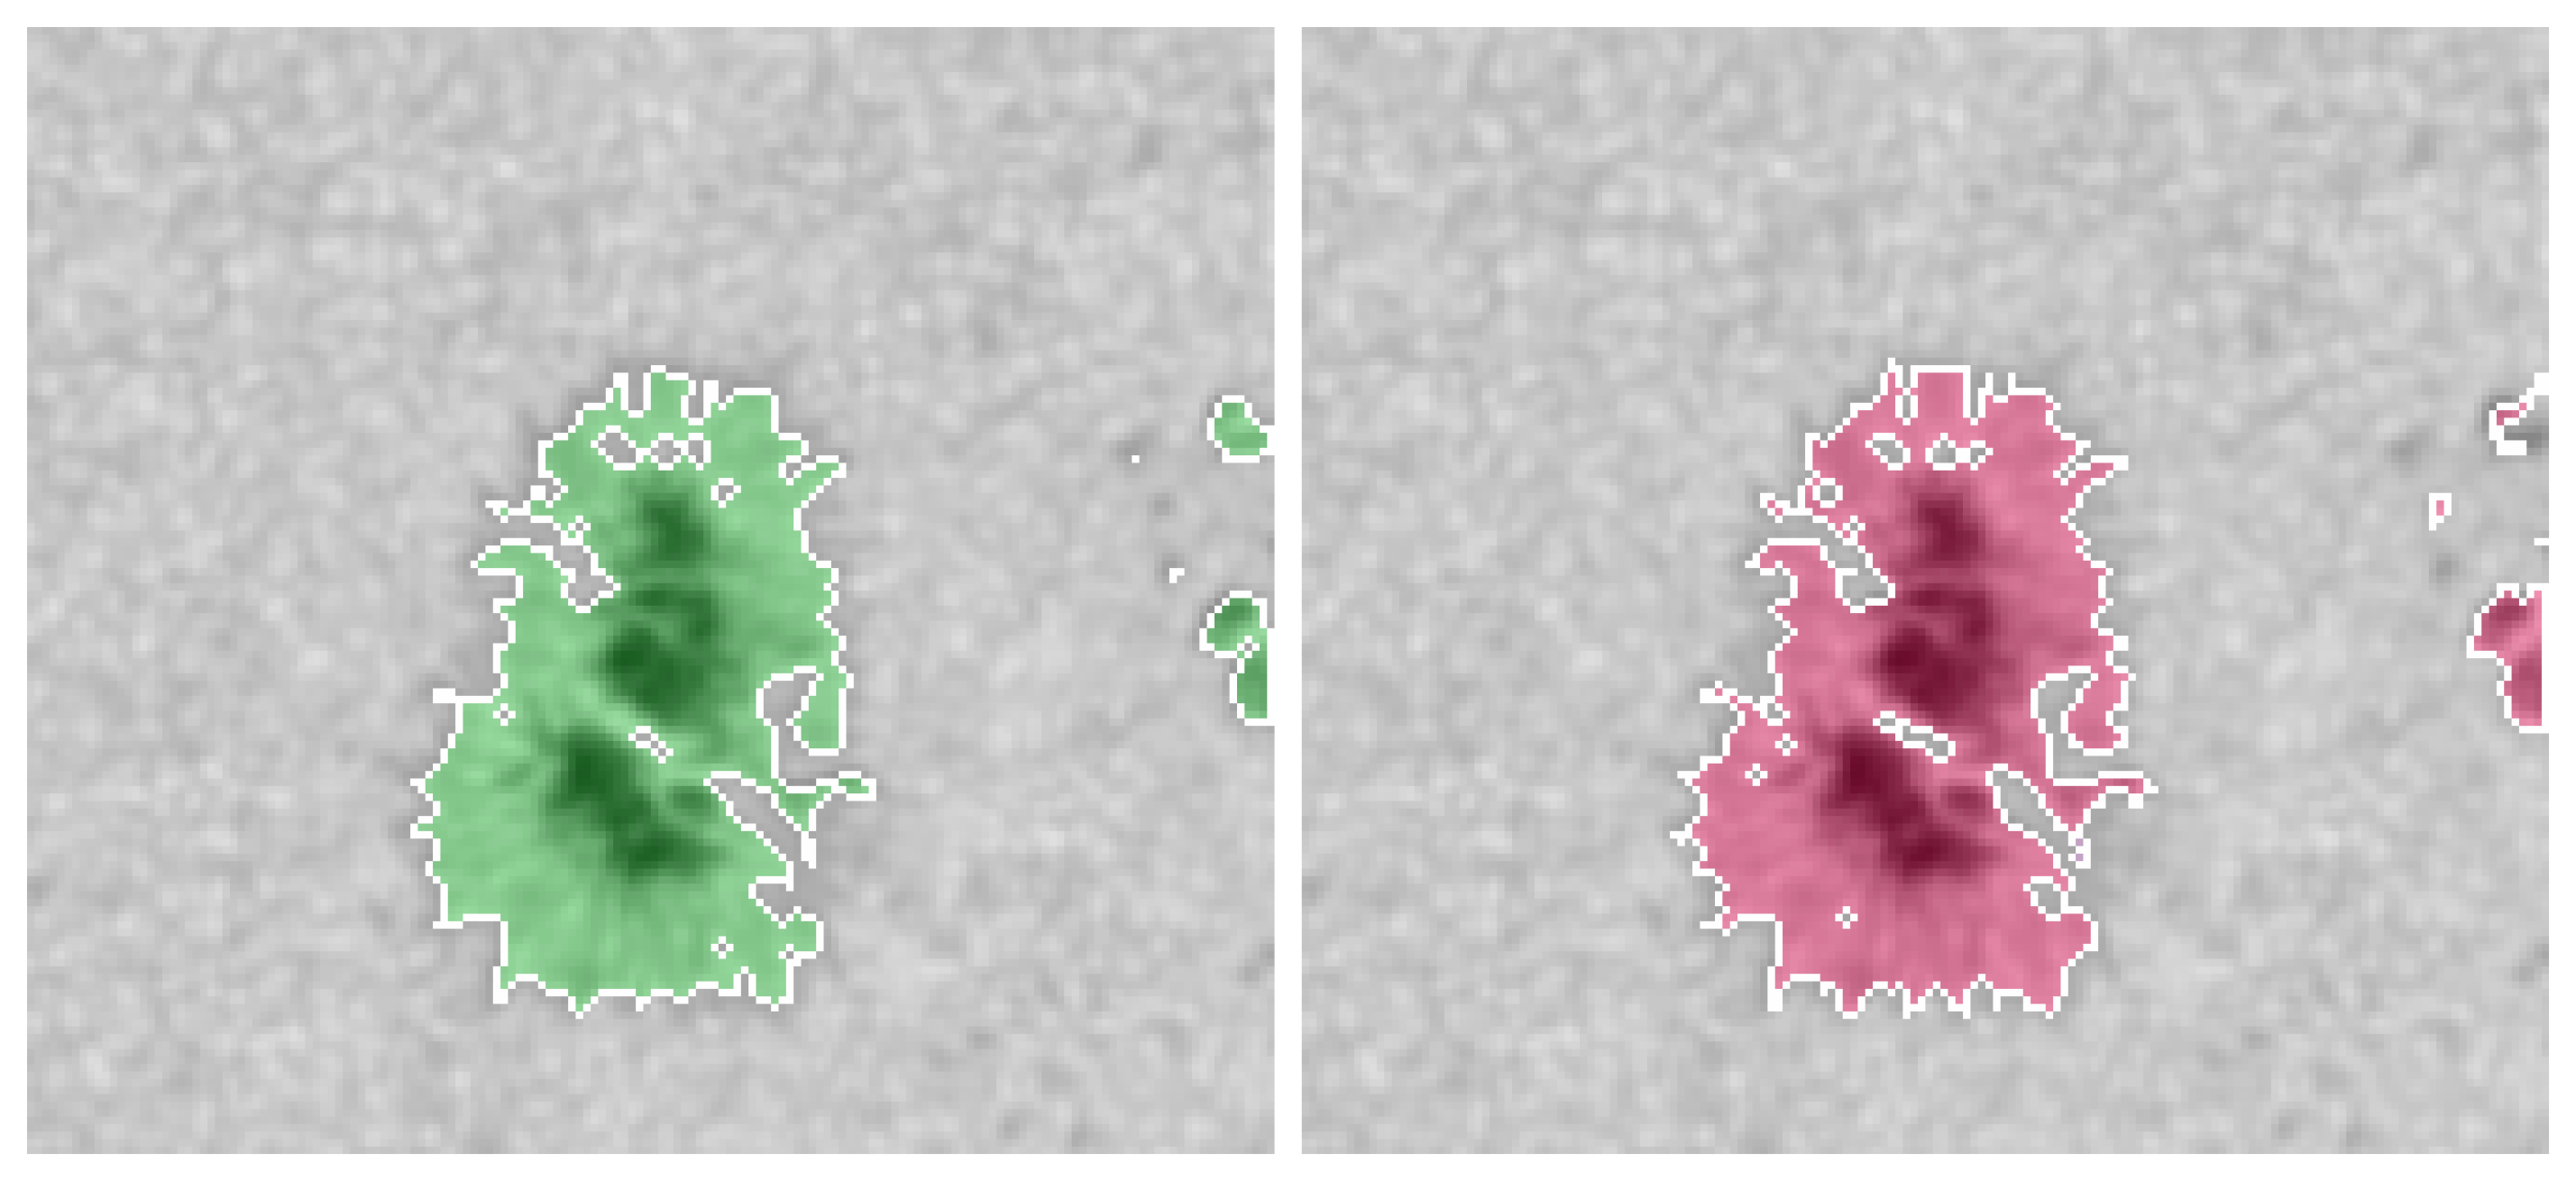
\includegraphics[width=\textwidth]{./pictures/pred-vs-ground}
    \caption{Comparison between the predicted mask (green) and the ground truth (red).}
    \label{fig:pred-vs-ground}
\end{figure}
\begin{figure}[t!]
    \centering
    \captionsetup{justification=centering}
    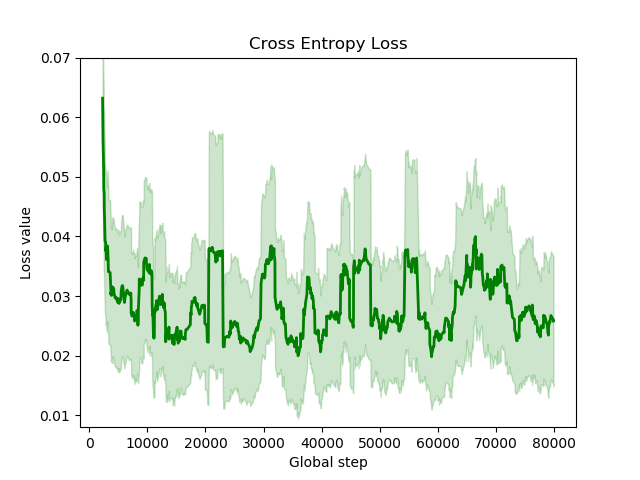
\includegraphics[width=\textwidth]{./pictures/cross-entropy-loss}
    \caption{U-Net convergence curve on the training set.}
    \label{fig:cross-entropy-loss}
\end{figure}
\clearpage
\begin{figure}[h]
    \centering
    \captionsetup{justification=centering}
    \includegraphics[width=\textwidth]{./pictures/workflow}
    \caption{Summary of the training of the segmentation phase}
    \label{fig:workflow}
\end{figure}
\clearpage
\subsection{Sunspot Representations and Classification}
Probably, the part of the sunspot index estimation that requires most expert knowledge is the determination of the number of groups. The setting of the problem is mainly unsupervised, because groups change every day and there is no predefined category that generalizes from one day to another.
\bigbreak
\noindent  Clustering seems a very natural approach for this problem. It is indeed, but it is also desirable to leverage the datasets of annotated sunspot groups that are available online to make the algorithm mimic the way humans cluster sunspots. A sensible form of blending together a supervised model with clustering is by using the labels to create good representations of the data. Specifically, we want to take the image of a sunspot and remap it to a feature vector that optimizes the result of the subsequent step. This can be achieved by training a siamese network that embeds sunspots in a way that separates them according to the configuration of the groups. To guide the neural network in the search of the optimal features to extract, a contrastive loss is applied. After the mapping is performed, clustering can be employed to find the number of groups.
\bigbreak
\noindent At each training episode a ground truth mask that also contains the instances of the clusters is loaded from the dataset. From every group that is present on the disk, an anchor sunspot is randomly chosen. If the sunspot is not alone in the group, a positive example is selected from the same group. Similarly, a negative example is chosen from the other clusters if they exist. A square patch is centered and cropped from the full-disk image for each example that has been sampled. Now, the visual appearence of the sunspot is certainly an important feature, but its position and its total area are crucial as well. So, how can we give this features as inputs to the siamese network? Recent studies have shown that coordinates can be given as input to convolutional neural networks to improve their performance \cite{liu2018intriguing}. Thus, the centroids of each sunspot in heliographic coordinates are appended as a channel to the input tensor (the coordinate value is repeated on the whole channel). The same is done with the value of the area, after having it normalized by the total area of the disk. The final input tensor to the convolutional layers has therefore 4 channels (as it can be seen in Figure~\ref{fig:siamese-workflow}) holding respectively:
\begin{itemize}
  \item 1 channel for the patch of the image that contains the sunspot;
  \item 2 channels for the heliographic latitude and longitude;
  \item 1 channel for the normalized area of the sunspot.
\end{itemize}
After the tensor is propagated, the convolutaional layers produce an intermediate representation that, in turn, passes through two fully connected layers, generating a 5-dimesional embedding as output. This procedure gets repeated for all the selected sunspots and for each one of them the loss tries to pull the positive matches together (low Euclidean distance) while pushing the negative ones apart (high Euclidean distance).
\bigbreak
\noindent At the same time, the convolutional layers are repurposed for classification. The intermediate representation generated by the convolutional layers is also fed to a second, almost identical fully connected block that deals with classification. In this case, the desired output is the modified Z\"{u}rich class (Z component of the McIntosh classification). Identifying the type of sunspot that is being processed is important because the presence of penumbra surrounding the umbra can be derived directly from the class. As always, the classification error (calculated with the standard cross entropy loss) is backpropagated through the layers. Note that the fully connected layers only receive the gradients coming from their own output while the shared convolutional layers accumulate the gradients coming from both the contrastive loss and the cross entropy loss.
\bigbreak
\noindent This type of learning paradigm, where the network solves two or more problems at the same time, is called multitask learning \cite{caruana1997multitask}. It is based on the idea that what is learned for each task can help other tasks be learned better. This is indeed the case for sunspot clustering. In fact, even humans use group classification as an aid in the process of grouping them together.
\bigbreak
\noindent The process of training this ``two-headed'' architecture was very hard, due to the fact that the way positive and negative examples are selected makes a very big impact on the final result. Nonetheless, finally, it was possible to make the network learn both tasks with very good performance. The training curves can be examined in Figure~\ref{fig:siamese-training}.
\begin{figure}[hb!]
  \centering
  \captionsetup{justification=centering}
  \includegraphics[width=\textwidth]{./pictures/siamese-workflow}
  \caption{Summary of the training of the siamese network}
  \label{fig:siamese-workflow}
\end{figure}
\begin{figure}[h!]
    \centering
    \captionsetup{justification=centering}
    \begin{subfigure}[t]{\textwidth}
        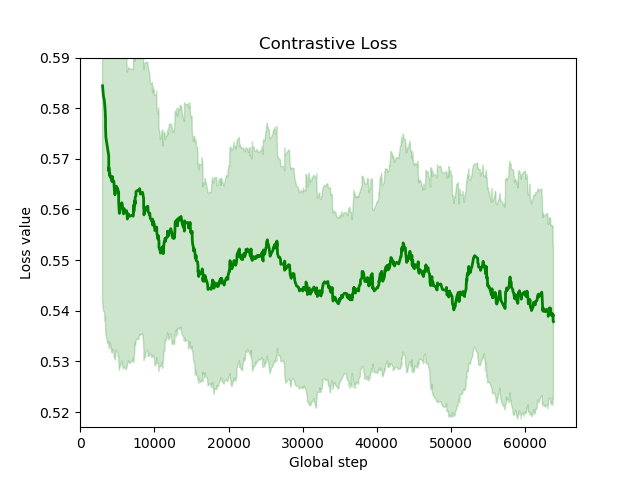
\includegraphics[width=\textwidth]{./pictures/contrastive-loss}
    \end{subfigure}\vspace{3mm}
    \begin{subfigure}[t]{\textwidth}
        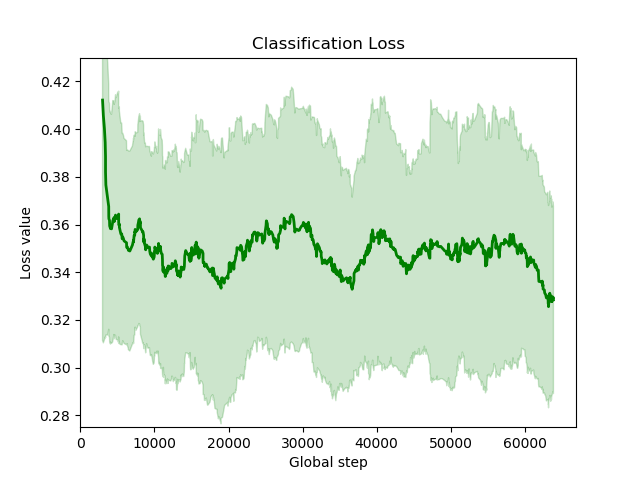
\includegraphics[width=\textwidth]{./pictures/classification-loss}
    \end{subfigure}
    \caption{Multitask siamese network convergence curve. Note that the implementation of the contrastive loss that has been used constrains the minimum possible value to be 0.5}
    \label{fig:siamese-training}
\end{figure}
\clearpage
\section{Automatic Annotation Procedure}
\label{autoannotation}
After both components of the model have been trained, it is time to join them in order to make predictions on unseen data. However, just stacking the U-Net and the siamese network together is not sufficient and other subcomponents are added. In this section we aim at describing in detail all the steps that are necessary to compose a successful annotation algorithm.
\bigbreak
\noindent Contrary to the training phase, the loading routine is now very simple, since it just needs to fetch the image that is annotated and no mask is needed (it is produced automatically). So, the prediction routine starts loading the image and dividing it into patches, while the parameters of the two neural networks get restored from selected checkpoints. One by one, the patches get sent into the U-Net that takes care of the first segmentation stage. As soon as the whole image has been evaluated, the mask gets reconstructed from the patches. Note that, since the U-Net outputs probabilities, every pixel has a continuous value (between 0 and 1) that needs to be rounded with a threshold in order to obtain a mask where the background has value 0 and the sunspot areas have value 1.
\bigbreak
\noindent At this point, we know with good confindence that the parts of the image that have been highlighted from the U-Net contain one or more sunspots each. To use this information for the subsequent steps we first need to convert it to a more usable form. The mask is, scanned looking for connected componets of pixels with value 1. At the same time, statistics are extracted for every component and the data is organized in an array. It is precisely from this information that the inputs for the siamese network are created. In fact, similarly to what was done during training time, the input channels are built using respectively a centered patch, the coordinates of the centroid and the area of the connected components. Coordinates are now in pixel space so they need to be translated to the heliographic system via trigonometry. When this is done, the data is forwarded through the convolutional layers of the siamese network and then the two fully connected heads are evaluated in parallel. The network outputs both the embeddings and the classes of each connected component.
\bigbreak
\noindent From this moment on, the computaton splits in two branches, one that seeks to refine the quality of the segmentation to yield the number of single sunspots, the other that finds the number of groups and assigns each sunspot to one of them.
\begin{figure}[ht!]
  \centering
  \captionsetup{justification=centering}
  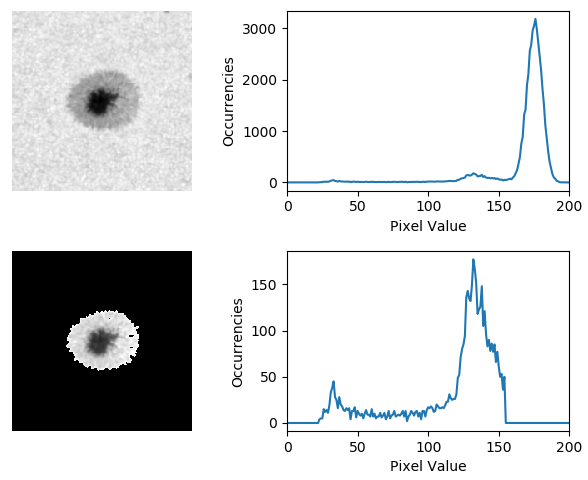
\includegraphics[width=\textwidth]{./pictures/histograms}
  \caption{Comparison between histograms of the same patch, with or without the mask}
  \label{fig:histograms}
\end{figure}
Refining the quality of the segmentation mask means, in this context, to be able to separate the umbra from the penumbra of each connected component of pixels generated by the U-Net. This operation is important because more than one umbrae can be surrounded by the same penumbrae, affecting the sunspot count. First, it is necessary to understand if the sunspot exhibits or not the penumbra. This is easy considered that we can leverage the classification produced by the siamese network together with some simple heuristic concerning the area of the sunspot.
\bigbreak
\noindent Classes \textbf{A} and \textbf{B} imply that the sunspots of the group do not have penumbra while classes \textbf{C} to \textbf{H} all expect penumbra. Small sunspots that usually locate at the periphery of groups are directly discarded with some threshold on the value of the area since we assume that they are very unlikely to carry more than one umbra. This knowledge enables us to segment the connected component using its histogram. In fact, since the division between umbra and penumbra creates a strong intensity discontinuity, the cut-off value is evident in the histogram if the mask of the whole sunspot is known a priori. Referring to Figure~\ref{fig:histograms} as an aid to visualization, the two peaks that can be seen around pixel value 30 and 130 are respectively the umbra and the penumbra. Given this knowledge of the problem we can proceed with two approaches, either fitting two gaussians and assigning each pixel to the most likely one, or simply perforoming clustering in one dimension fixing the number of clusters to the value 2. Both solutions were explored during the development of this work but in the end clustering was selected because, despite being simpler, it yields the same performance.
\bigbreak
\noindent At the end, the refinement of the segmentation step reduces to running k-means on the mask generated by the U-Net. The two clusters of pixels are then used to create a new mask that only highlights umbras, and the number of connected components is recalculated from it.
\bigbreak
\noindent The second branch of the procedure finds the number of groups and assigns each sunspot (connected component of pixels) to one of them, using the embeddings created by the siamese network. Those embeddings are created to optimize the positions of the connected components in a 5-dimensional Euclidean space. As already treated in the previous section, the optimization operated by the siamese network lies in the fact that sunspots belonging to the same group should be close together in the Euclidean space. This is, once again, a great opportunity to unleash the potential of clustering algorithms. However, the main difficulty here is that the number of clusters is not known beforehand, because it is indeed the value that we want to calculate.
\bigbreak
\noindent DBSCAN seems like a very good match for this problem. In fact, it just needs two parameters: $eps$ ($\varepsilon$) which can be estimated statistically on the validation set (see next section) and $minPts$ which is trivially set to 0 (otherwise groups composed by a lone sunspot would be interpreted as outliers). Given the parameters and the embeddings as inputs, DBSCAN reliably returns the number of clusters that is useful for later computations.
\bigbreak
\noindent Now that the image has been annotated and the number of groups and single sunspots is known it is sufficient to find the personal reduction coefficient to be able to calculate the final value of the relative sunspot number. The estimation of the personal reduction coefficient and the $eps$ ($\varepsilon$) parameter for DBSCAN are addressed in the next section.

\section{Parameter Estimation}
The validation set provides an exceptional opportunity for the estimation of parameters. In fact, many instances of the algorithm can be run using the data that was held out from the training set, so the variation in performance can be assessed. Various combinations of parameters can be evaluated and the best model can be then used to draw the final results on the test set.
Among the others, two parameters have been studied in detail in this work:
\begin{itemize}
  \item the $eps$ ($\varepsilon$) parameter for DBSCAN that represent the minimum distance between two points for them to be considered neighbors;
  \item the personal reduction coefficient ($K$) of the algorithm, compared to the international sunspot number provided by SILSO.
\end{itemize}
These two parameters are not independent from each other and therefore they were tested in two consecutive phases, both on the whole validation set.
\bigbreak
\noindent The first one that needed to be assessed was the value of $eps$. The number of clusters detected from DBSCAN dramatically depends on this parameter, so optimizing it is vital to improve the final performance. Although the variable that drives the performance is the number of clusters, we didn't use it as the measure to optimize $eps$ because it is not informative enough. Instead, the Adjusted Random Index (ARI), a performance index that takes into account the configuration of points inside the clusters and compares it to the ground truth was used. ARI is defined as:
\begin{equation}
ARI = \frac{RI-\mathbb{E}[RI]}{max(RI)-\mathbb{E}[RI]}
\end{equation}
where $RI$ (Rand Index) is the number of pairs of objects that are either in the same group or in different groups in both partitions divided by the total number of pairs of objects. The ARI performs a correction with respect to the Rand index in order to account for the variability of the expected value of two random partitions. Thus, the ARI has a value close to 0 for random labeling independently of the number of clusters and exactly 1 when the clusterings are identical.
\bigbreak
\noindent We tested the algorithm 50 times on the whole validation set, each time with a different value for the $eps$ parameter. The results are shown in Figure~\ref{fig:eps-ari}. After the estimation of the curve it is possible to take the value that maximizes the performance index and use it as input for the subsequent tests.
\bigbreak
\noindent After $eps$, we proceded to estimate the value of the reduction coefficient $K$ using a similar procedure. This time, instead of maximizing some performance index, the task is to minimize the deviation of our calculation of the sunspot number from the international sunspot index provided by SILSO. This can be achieved using the root-mean-square (RMS) error between the two calculations over the whole validation set. The procedure was repeated 100 times with values of $K$ ranging from 0 to 2 (Figure~\ref{fig:k-rms}). The optimal minimal error is attained when the $K$ coefficient takes the value 0.58. Such a low value for $K$ is explained by the fact that the images that have been used by our algorithm come from the best observatories in the world. Depending on the optics of the telescope, the amount of detail that can be resolved changes. So, in general, the better the optics, the more sunspots it captures. For this reason, the estimation our algorithm provides is high, and therefore it should be multiplied by a low value to align to the international sunspot number.\clearpage
\begin{figure}[ht!]
  \centering
  \captionsetup{justification=centering}
  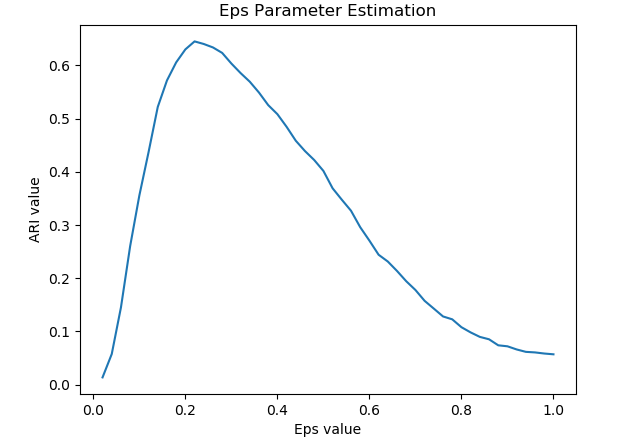
\includegraphics[width=\textwidth]{./pictures/eps-ari-copy}
  \caption{ARI value for varying $eps$ values}
  \label{fig:eps-ari}
\end{figure}
\begin{figure}[h!]
  \centering
  \captionsetup{justification=centering}
  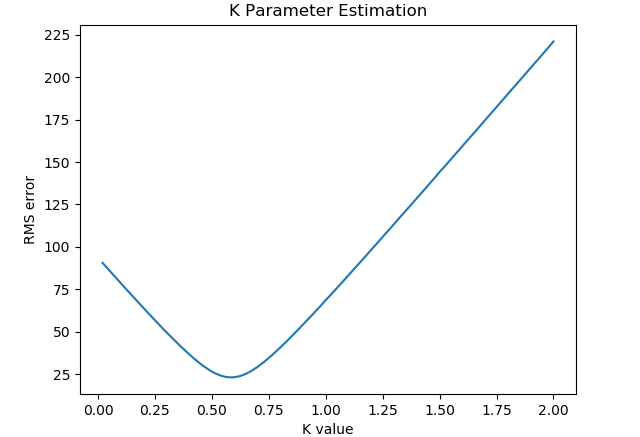
\includegraphics[width=\textwidth]{./pictures/k-rms-copy}
  \caption{RMS error value for varying $K$ value}
  \label{fig:k-rms}
\end{figure}
